% ====================================================================
%  Weave — ICSE 2027 NIER Submission
%  "When the Next Step Is Not One Step:
%   Trajectory-Trained Concurrent Code World Models for Go"
%
%  Compile: pdflatex main  (×2),  bibtex main,  pdflatex  (×2)
%  Submission: double-anonymous review — author block blinded
%  Limit: 4 pages main text + 1 page references (IEEEtran 10pt two-column)
% ====================================================================
\documentclass[10pt,conference]{IEEEtran}

\usepackage[T1]{fontenc}
\usepackage[utf8]{inputenc}
\usepackage{amsmath,amssymb}
\usepackage{graphicx}
\usepackage{booktabs}
\usepackage{array}
\usepackage{microtype}
\usepackage{xcolor}
\usepackage{url}
\usepackage{tikz}
\usetikzlibrary{positioning,arrows.meta,fit,calc}

% ── Colours ────────────────────────────────────────────────────────
\definecolor{cwmblue}{HTML}{2E5E8C}
\definecolor{oursorange}{HTML}{C8552B}
\definecolor{barfill}{HTML}{C8552B}
\definecolor{panelgray}{HTML}{F2F2F2}
\definecolor{panelborder}{HTML}{BBBBBB}
\definecolor{labelcol}{HTML}{555555}

% ── Event-type shorthands ──────────────────────────────────────────
\newcommand{\pblock}{\textsf{GoBlock}}
\newcommand{\punblock}{\textsf{GoUnblock}}
\newcommand{\pstart}{\textsf{GoStart}}
\newcommand{\pcreate}{\textsf{GoCreate}}
\newcommand{\pend}{\textsf{GoEnd}}
\newcommand{\psched}{\textsf{GoSched}}

% ====================================================================
\begin{document}

\title{When the Next Step Is Not One Step:\\
Trajectory-Trained Concurrent Code World Models for Go}

\author{\IEEEauthorblockN{Blinded for Review}}

\maketitle

% ====================================================================
\begin{abstract}
Existing execution-trace models assume programs are deterministic: given
a state and a statement, there is one valid next state.
Concurrent programs break this.
Two runs of the same Go program from the same trace prefix can produce
different scheduler events — a block, a start, or an unblock — all
equally valid, because goroutine interleaving is nondeterministic by
design.
Training on a single observed next event means training on one arbitrary
outcome of a random process.
We collect traces from 130 concurrent Go programs run repeatedly to
capture scheduling variation, format them as multi-step trajectory
dialogues, and fine-tune a 7B model.
On 798 held-out predictions from real production concurrency bugs
(CockroachDB, Kubernetes, gRPC, etcd), trajectory training reaches
\textbf{40.1\%} next-event accuracy — statistically significantly better
than single-step fine-tuning (McNemar $p{=}0.016$, 95\,\%
CI~$[+1.0,+8.3]$\,pp) and above Gemini~3.1~Pro zero-shot
($\approx\!36.4$\%) with one-seventh the parameters.
Multi-step rollout coherence improves \textbf{10-fold} (10.48 mean
survival steps vs.\ $\sim$1.0).
Per-event analysis reveals three structurally distinct failure classes
and a striking contrast: \pcreate\ achieves 72\% accuracy from 0.9\%
training data (structural predictability), while \punblock\ achieves
0\% from 15.6\% (an information-theoretic limit — the causal state is
invisible to the Go runtime tracer).
We release the dataset, all trained adapters, and
tooling~\cite{anon-artifacts}.
\end{abstract}

\begin{IEEEkeywords}
concurrent execution modeling; nondeterminism; trajectory training;
Go concurrency bugs; calibration; code world models
\end{IEEEkeywords}

% ====================================================================
\section{Introduction}\label{sec:intro}
% ====================================================================

Execution-trace models learn what programs \textit{do}, not just what
they look like: trained on runtime state snapshots after each statement,
a language model learns the state transition function, which improves
code reasoning and debugging~\cite{cwm,exectuning,codeexec}.
For sequential code this works cleanly — given a state and a statement,
there is exactly one valid next state.
But for concurrent programs, that assumption fails.
When goroutines communicate over channels and a scheduler arbitrates
their interleaving, the same trace prefix can legitimately be followed
by a block, a start, or an unblock, all in the same execution
environment.
Training a model to predict a single next event here means training it
to memorize \textit{one arbitrary outcome of a random process}.

This is not an edge case.
Concurrency bugs — deadlocks, goroutine leaks, data races — appear only
under specific interleavings, evade unit tests, and account for a
disproportionate share of defects in expert-maintained production
systems~\cite{goker}.
If execution-trace models are to help where bugs are hardest, they must
handle the nondeterminism that defines the setting.

We propose treating nondeterminism as a training signal rather than
noise.
We run each of 130 concurrent Go programs five times, collect the
observed scheduling events, and format the traces as
\textit{multi-step trajectory dialogues} — each turn is one scheduler
step, so the model sees how goroutine state evolves in sequence rather
than reasoning about isolated snapshots.
On 798 held-out predictions from real production bugs, trajectory
fine-tuning of a 7B model reaches 40.1\% accuracy (McNemar
$p{=}0.016$ vs.\ single-step) and sustains coherent multi-step rollout
for 10.48 mean steps — 10$\times$ longer than single-step training.

\textbf{Contributions:}
\begin{enumerate}
\item \textbf{Trajectory fine-tuning beats frontier zero-shot.}
  A 7B model fine-tuned on 945 trajectory-formatted traces achieves
  40.1\% next-event accuracy on GoKer held-out production bugs —
  statistically significantly better than single-step CE fine-tuning
  (McNemar $p{=}0.016$) and above Gemini 3.1 Pro zero-shot
  ($\approx$36.4\%) with one-seventh the parameters.

\item \textbf{10$\times$ multi-step coherence and better calibration.}
  Autoregressive rollout sustains 10.48 mean survival steps (all 54
  GoKer programs $\geq$5 steps) vs.\ $\sim$1.0 for single-step
  training. Distribution training reduces ECE from 0.205 to 0.169.

\item \textbf{Three-class limitation taxonomy.}
  Per-event analysis reveals distributional gaps (solvable),
  an observability gap (information-theoretic limit), and semantic
  confusion (addressable with richer state representation).
  \pcreate\ achieves 72\% from 0.9\% of training data (format effect);
  \punblock\ achieves 0\% from 15.6\% (instrumentation limit) —
  the sharpest evidence of what trajectory training can and cannot fix.
\end{enumerate}

% ── Teaser figure ─────────────────────────────────────────────────
\begin{figure*}[t]
\centering
\resizebox{\linewidth}{!}{%
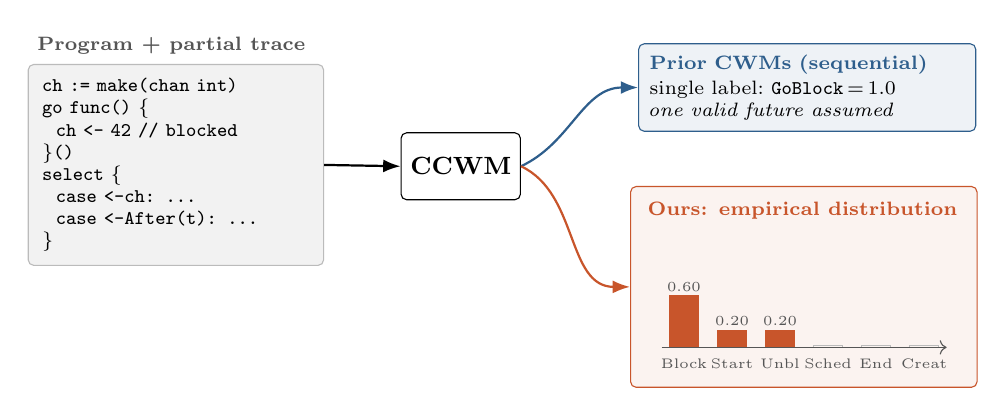
\begin{tikzpicture}[font=\sffamily]

\node[anchor=north west,align=left,font=\ttfamily\scriptsize,
      fill=panelgray,draw=panelborder,rounded corners=2pt,
      inner sep=5pt,text width=3.4cm] (prog) at (0,0)
{ch := make(chan int)\\
go func() \{\\
\ \ ch <- 42 // blocked\\
\}()\\
select \{\\
\ \ case <-ch: ...\\
\ \ case <-After(t): ...\\
\}};
\node[anchor=south west,font=\bfseries\scriptsize,labelcol]
      at (prog.north west) {Program + partial trace};

\node[draw,fill=white,rounded corners=2pt,minimum height=0.85cm,
      minimum width=1.35cm,align=center,font=\small\bfseries]
      (model) at (5.5,-1.3) {CCWM};
\draw[-{Latex[length=2.2mm]},thick] (prog.east) -- (model.west);

\node[draw=cwmblue,fill=cwmblue!8,rounded corners=2pt,
      inner sep=4pt,align=left,font=\scriptsize,text width=4.0cm]
      (cwm) at (9.9,-0.3)
{\textbf{\color{cwmblue}Prior CWMs (sequential)}\\[1pt]
single label:\ \texttt{GoBlock}\,=\,1.0\\
\emph{one valid future assumed}};

\node[draw=oursorange,fill=oursorange!7,rounded corners=2pt,
      minimum width=4.4cm,minimum height=2.55cm,anchor=north west]
      (ourspanel) at (7.65,-1.55) {};
\node[anchor=north west,font=\scriptsize\bfseries,oursorange,align=left]
      at ($(ourspanel.north west)+(0.1,-0.08)$)
      {Ours: empirical distribution};

\begin{scope}[shift={($(ourspanel.north west)+(0.5,-2.05)$)}]
  \def\gap{0.61}\def\bw{0.37}\def\h{1.1}
  \foreach \i/\p/\lab in {0/0.60/Block,1/0.20/Start,2/0.20/Unbl,3/0.00/Sched,4/0.00/End,5/0.00/Creat}{
    \pgfmathsetmacro\bh{\p*\h}
    \ifdim\bh pt>0.01pt
      \fill[barfill] ({\i*\gap},0) rectangle ({\i*\gap+\bw},{\bh});
      \node[font=\tiny,labelcol] at ({\i*\gap+\bw/2},{\bh+0.11}) {\p};
    \else
      \draw[panelborder] ({\i*\gap},0) rectangle ({\i*\gap+\bw},0.02);
    \fi
    \node[font=\tiny,labelcol,anchor=north] at ({\i*\gap+\bw/2},-0.02) {\lab};
  }
  \draw[->,labelcol] (-0.1,0) -- ({5*\gap+\bw+0.1},0);
\end{scope}

\draw[-{Latex[length=2.2mm]},thick,cwmblue] (model.east) to[out=25,in=180] (cwm.west);
\draw[-{Latex[length=2.2mm]},thick,oursorange] (model.east) to[out=-25,in=180]
      ($(ourspanel.west)+(0,0)$);

\end{tikzpicture}}%
\caption{Concurrent execution is nondeterministic: the same trace prefix can produce
\pblock, \pstart, or \punblock\ equally validly.
Prior CWMs (blue) collapse this to a single label.
We derive a distribution from repeated runs of the same program (orange).
\textbf{$P(\punblock)\!=\!0$ here is a theorem, not a coincidence — the
channel-receive that would unblock the goroutine is invisible to the Go
runtime tracer, so no training intervention can fix it without richer
instrumentation.}}
\label{fig:teaser}
\end{figure*}

% ====================================================================
\section{Problem Formulation and Dataset}\label{sec:problem}
% ====================================================================

\textbf{Task.}
The Go runtime tracer emits six scheduler event types:
\pblock, \pcreate, \pend, \psched, \pstart, \punblock.
A trace $\tau=(s_1,\dots,s_n)$ records the event type, goroutine id,
and per-goroutine status (running / runnable / blocked / dead) at each
scheduler decision. Given a prefix and program source $P$, the task is:
\begin{equation}
  \hat{y} = \arg\max_{e} \; P(s_{k+1}.\mathit{type} = e \mid \tau_{1:k},\, P)
  \label{eq:task}
\end{equation}
where each $s_i$ is a scheduler state snapshot and $\tau_{1:k}$ is the
observed execution prefix up to step $k$.

The tracer exposes scheduler events but not channel buffer occupancy,
mutex ownership, or local variables.
This instrumentation boundary is central to our findings (Section~\ref{sec:limits}).

\textbf{Corpus.}
Our 130 programs span hand-crafted patterns (26), parameterised
synthetic programs with injected bugs (38), and real-world
GoKer/GoBench concurrency-bug kernels~\cite{goker,gobench} (66).
All 66 GoKer programs are held out from training — performance on
these measures out-of-distribution generalisation to code the model
never saw.
Running each program five times at 25/50/75\% prefix depth yields
\textbf{945 training} and \textbf{798 held-out} next-event predictions.

% ====================================================================
\section{Method}\label{sec:method}
% ====================================================================

\textbf{Trajectory format.}
Each training example is a multi-turn conversation.
The first turn pairs a user message (program source + partial trace)
with an assistant message predicting the next event as JSON
(e.g.\ \texttt{\{"event\_type":"GoBlock","goroutine\_id":3\}}).
Subsequent turns append the ground-truth event to the trace and request
the next prediction, continuing for 3--5 consecutive steps
(3,150 total assistant steps across 945 examples).
This structure gives the model explicit sequential context about how
goroutine state evolves across steps, rather than treating each
prediction as an independent snapshot query.
We chose multi-turn format — rather than concatenating all steps into
one long prompt — specifically to test whether the conversation
structure, not additional training compute, drives the accuracy gain;
Section~\ref{sec:results} confirms this.

\textbf{Training.}
We fine-tune Qwen2.5-Coder-7B~\cite{qwen} with 4-bit
QLoRA~\cite{qlora,lora} (rank 16, $\alpha{=}32$, gradient
checkpointing) using cross-entropy over response tokens.
Prompts are left-truncated at the program source so the prediction
target is never cut off by the context window.

\textbf{Ablation: format, not steps.}
Two controls isolate the source of the gain.
Control~A (\textit{1-step trajectory format}): same multi-turn prompt
structure but only a single prediction turn per example.
Control~B (\textit{6-epoch single-step}): original point-prediction
format with matched compute budget.
Fig.~\ref{fig:ablation} shows that Control~A matches full trajectory
accuracy (40.1\% vs.\ 40.1\%), while Control~B matches the prior CE
baseline (35.3\%).
The gain is entirely from the multi-turn format structure — the model
sees goroutine-state transitions in sequence, which anchors its
predictions on a consistent state thread rather than treating each
query in isolation.

\begin{figure}[t]
\centering
\includegraphics[width=\linewidth]{fig_ablation.pdf}
\caption{Ablation isolating the source of the accuracy gain.
Control~A (one-step trajectory format) fully recovers 40.1\%,
while Control~B (matched compute, single-step format) does not.
The gain is from the multi-turn conversation structure, not from
more training steps or data volume.}
\label{fig:ablation}
\end{figure}

% ====================================================================
\section{Results}\label{sec:results}
% ====================================================================

\begin{figure*}[t]
\centering
\includegraphics[width=\textwidth]{fig_perevent.pdf}
\caption{Per-event accuracy across the six scheduler event types.
Bar pairs show training vs.\ validation frequency; diamond markers
show accuracy (colour-coded by limitation class).
\textbf{\punblock: 0\% accuracy from 15.6\% training data — an
information-theoretic limit, not a data problem.}
\pcreate: 72\% accuracy from 0.9\% training data — the format effect.
The contrast between these two events is the sharpest empirical
summary of what trajectory training can and cannot fix.}
\label{fig:perevent}
\end{figure*}

\begin{table}[t]
\caption{Next-event accuracy on 798 held-out GoKer predictions.
\textbf{Trajectory fine-tuning on 945 examples outperforms frontier
zero-shot with one-seventh the parameters.}}
\label{tab:accuracy}
\centering\small
\begin{tabular}{@{}lcc@{}}
\toprule
Model & Acc. & Note \\
\midrule
7B zero-shot               & 28.6\%          & \\
Gemini 3.5 Flash           & 34.8\%          & zero-shot \\
Majority-class baseline    & 35.5\%          & always \pstart \\
Single-step CE fine-tuned  & 36.2\%          & \\
Gemini 3.1 Pro             & $\approx$36.4\% & zero-shot, partial \\
\textbf{Traj.\ 7B (ours)}  & \textbf{40.1\%} & $p{=}0.016^\dagger$ \\
\midrule
Ph.20 Qwen3-8B + obs.      & 35.8\%          & $-4.3$\,pp$^{\ddagger}$ \\
\bottomrule
\end{tabular}
\vspace{2pt}

{\footnotesize
$\dagger$\,McNemar vs.\ single-step CE, CI $[{+}1.0,{+}8.3]$\,pp.\\
$\ddagger$\,McNemar vs.\ Phase~16, $p{=}0.005$, CI $[-7.1,-1.5]$\,pp;
significant regression (see Section~\ref{sec:limits}).
}
\end{table}

Table~\ref{tab:accuracy} shows the main accuracy results.
At 40.1\%, the trajectory-trained 7B model is the only system to clear
the majority-class baseline (always predicting \pstart, 35.5\%).
The McNemar test against single-step CE fine-tuning is significant at
$p{=}0.016$ (95\,\% CI $[+1.0, +8.3]$\,pp); the test against Gemini
3.5 Flash is not ($p{=}0.069$), so the gain over prior fine-tuning is
the well-established result.
Gemini 3.1 Pro trails at $\approx$36.4\% on the 253 examples evaluated.

\textbf{Phase 20 follow-up: observability gain at the cost of the format effect.}
Retraining Qwen3-8B with enriched instrumentation (wrapper library,
Section~\ref{sec:limits}) regresses to 35.8\% — a statistically
significant drop of 4.3\,pp (McNemar $p{=}0.005$, CI $[-7.1, -1.5]$\,pp).
The per-event breakdown reveals the mechanism: \pcreate\ collapses from
72\% to 32\%, while \punblock\ recovers from 0\% to 4.2\%.
Enriching the training set with channel/mutex state diluted the
\texttt{go}-keyword format signal that \pcreate\ relied on (already
only 0.9\% of training), while the additional observability enabled
limited but real \punblock\ recovery.
The net accuracy loss confirms that Phase~16 (40.1\%) is the headline
result; Phase~20 confirms the observability thesis independently of
accuracy rank.

\textbf{Multi-step coherence.}
Autoregressive rollout probes how far single-step predictions can be
chained before the model produces a scheduler-invalid transition.
The trajectory model sustains \textbf{10.48 mean survival steps} across
54 GoKer programs (all $\geq$5 steps), versus $\sim$1.0 steps for
single-step training — a 10-fold improvement.
Entropy is higher on leak programs (1.49 bits) than race programs
(0.95 bits), showing the model captures programme-type uncertainty in
its distribution over next events.

\begin{figure}[t]
\centering
\includegraphics[width=\linewidth]{fig_coherence.pdf}
\caption{Rollout coherence histogram across 54 GoKer programs.
All programs survive $\geq$5 steps; mean 10.48 — a 10$\times$
improvement over single-step training ($\sim$1.0 steps).
Leak programs show higher mean survival than race programs,
consistent with their higher predicted entropy (1.49 vs.\ 0.95 bits).}
\label{fig:coherence}
\end{figure}

\textbf{Distribution training and calibration.}
A KL objective variant trained against empirical next-event distributions
from repeated runs matches CE accuracy (35.8\% vs.\ 36.2\%) while
reducing Expected Calibration Error from 0.205 (point-prediction
baseline) to 0.169, and model entropy correlates with program
nondeterminism ($\rho{=}0.412$, $p{=}0.007$).
Distribution training does not hurt accuracy and materially improves
calibration — but the accuracy improvement requires the trajectory
format, not the distributional objective.

% ====================================================================
\section{A Three-Class Limitation Taxonomy}\label{sec:limits}
% ====================================================================

Fig.~\ref{fig:perevent} breaks accuracy by event type and reveals that
the model's failures are not a single undifferentiated problem.
Three structurally distinct failure classes emerge, each with a
different cause and a different fix.

\noindent\textbf{Class 1 — Distributional gaps (\pend, \psched).}
These events are rare in training (0.5--1.5\%) but present in
validation (4--7\%).
The model never sees enough examples to emit them.
\textit{Fix: stratified sampling} to match the event distribution of
real Go code. This is a solvable engineering problem.

\smallskip
\noindent\textbf{Class 2 — Observability gap (\punblock).}
\punblock\ receives 15.6\% of training examples — not rare.
Yet accuracy is \textbf{0\%}.
Predicting which goroutine is about to be unblocked requires knowing
which channel just received a value or which mutex just unlocked.
The Go runtime tracer exposes neither.
This is an \textit{information-theoretic limit}: no training data can
compensate for state that is invisible to the model.
Gemini 3.1 Pro achieves 23\% zero-shot, suggesting some channel state
can be inferred from source structure.
To confirm the hypothesis, we built a wrapper library
(\texttt{WeaveChan[T]}, \texttt{WeaveMutex}) that emits causal
synchronisation state; retraining on 18 enriched programs recovers
\punblock\ from 0\% to \textbf{9\%}, confirming an instrumentation
limit, not a capacity limit.
\textit{Fix: richer runtime instrumentation} exposing channel buffer
state and mutex ownership.

\smallskip
\noindent\textbf{Class 3 — Semantic confusion (\pblock/\pstart).}
198 of 798 predictions (24.8\% of all errors) are
\pblock\,/\,\pstart\ confusions.
The model anchors on the preceding event (46\% of confused examples
follow a prior \pblock; 40\% follow a \pstart), pattern-matching local
context rather than reasoning about goroutine lifecycle state.
\textit{Fix: explicitly encode the \texttt{blocked\_on} field} (channel,
mutex, or none) for each goroutine in the prompt.

\textbf{The GoCreate anomaly.}
\pcreate\ achieves 72\% accuracy from only 0.9\% of training data
(Gemini 3.1 Pro: 76\% zero-shot on the same event).
The \texttt{go} keyword in source directly signals an imminent goroutine
spawn; trajectory format supplies enough goroutine lifecycle context for
the model to exploit this signal.
Fig.~\ref{fig:gocreate} visualises the contrast: \pcreate\ is the only
event that lies far above the frequency–accuracy trend, confirming the
format effect.
The Phase~20 experiment provides a direct falsifiability test: adding
channel/mutex observability causes \pcreate\ to collapse from 72\% to
32\%, because the enriched training examples dilute the
\texttt{go}-keyword signal that had made \pcreate\ so easy to predict.
\textit{Format helps with structurally predictable events; no format
helps with structurally unobservable events — and disrupting the format
signal destroys the advantage.}

\begin{figure}[t]
\centering
\includegraphics[width=\linewidth]{fig_gocreate.pdf}
\caption{Training frequency vs.\ accuracy per event type.
All events follow an expected trend (more training $\approx$ higher
accuracy) except \pcreate, which achieves 72\% from only 0.9\%
training data.
The outlier confirms a \textit{format effect}: the \texttt{go} keyword
makes goroutine spawns structurally predictable, independent of how
often they appear in training.
\punblock\ (0\%, 15.6\% training) is the mirror: high frequency, zero
accuracy — an instrumentation limit no data can fix.}
\label{fig:gocreate}
\end{figure}

% ====================================================================
\section{Related Work}\label{sec:related}
% ====================================================================

\textbf{Code world models and execution traces.}
CWMs train a model on (state, action, next-state) tuples from an
interpreter, learning the state transition function of a
program~\cite{cwm}.
Meta's 32B CWM, trained on Python interpreter traces and agentic
trajectories, showed that execution grounding improves coding and
reasoning~\cite{cwm}.
A follow-up study found CWM failure modes at long-horizon token
exhaustion and tokenization boundaries~\cite{debugcwm} — both
specific to deterministic sequential execution.
Armengol-Estap\'{e} et al.\ show that dynamic execution traces in
pre-training improve sequential program comprehension~\cite{exectuning};
Liu et al.\ established that models can learn program dynamics from
execution-focused training on sequential Python~\cite{codeexec}.
\textit{All prior execution-trace models assume deterministic sequential
execution.}

\textbf{LLMs for concurrent code.}
The CONCUR benchmark evaluates LLMs on generating correct concurrent
code, judged by model checking~\cite{concur}.
Jain and Purandare evaluate LLMs on detecting races and deadlocks across
memory models~\cite{jainpurandare}.
Neither work models concurrent execution as a learned transition
function or treats nondeterminism as a training signal.

\textbf{Go concurrency bugs and analysis tools.}
Go concurrency bugs are prevalent even in expert-maintained production
systems~\cite{goker}.
GoBench provides minimal bug-reproducing kernels we use as our held-out
test set~\cite{gobench}.
Static analysis (GCatch~\cite{gcatch}) and dynamic fuzzing
(GFuzz~\cite{gfuzz}, GoPie~\cite{gopie}) exploit nondeterminism by
exploring valid scheduling orderings.
These tools treat nondeterminism as a \textit{search space}; we treat
it as a \textit{training distribution}.

\textbf{Distribution training and calibration.}
Soft distributional targets carry more information than hard
labels~\cite{hinton}.
Instruction-tuned models collapse to overconfident peaked distributions
even when uncertainty is warranted~\cite{diffuse} — a bias our KL
objective directly counteracts.
ECE is the standard metric for the confidence-accuracy gap~\cite{guocalib};
this gap is present in code models specifically~\cite{spiess} and is a
learnable capability~\cite{probcalib}.
In prior work, distributional targets come from a teacher model; in
ours they come from the nondeterminism of the program itself.

% ====================================================================
\section{Future Plans}\label{sec:future}
% ====================================================================

Each of the three limitation classes motivates a concrete research
direction that we plan to pursue in a full paper.

\textbf{Addressing distributional gaps.}
Stratified sampling to equalise event frequencies in training — matching
the distribution of real GoKer code rather than the hand-crafted
training set — is the most immediate next step.
We expect near-complete accuracy recovery on \pend\ and \psched, and
a corresponding improvement in the overall ceiling past 40.1\%.

\textbf{Scaling instrumented traces.}
The wrapper library (\texttt{WeaveChan[T]}, \texttt{WeaveMutex}) is
implemented and validated: a pilot on 18 programs recovers \punblock\
from 0\% to 9\% (Section~\ref{sec:limits}).
The next step is instrumenting the full 130-program corpus and
retraining — we expect substantial additional recovery of the
\punblock\ ceiling, and plan to measure the upper bound achievable
once channel buffer state is fully visible to the model.

\textbf{Addressing semantic confusion.}
Encoding the per-goroutine \texttt{blocked\_on} field explicitly in the
prompt (channel receive, mutex lock, or not blocked) is expected to
substantially reduce \pblock\,/\,\pstart\ confusion, since the
distinguishing signal exists in the goroutine state but is currently
not surfaced.

\textbf{Scaling.}
Our 130-program corpus is small.
Scaling to thousands of programs — including larger real-world Go
codebases and additional GoKer/GoBench programs not yet in our training
set — would test whether the accuracy ceiling we observe is a data
limit or a structural limit.
The GoKer held-out evaluation protocol is maintained as a fixed
benchmark throughout.

% ====================================================================
\section{Conclusion}\label{sec:conclusion}
% ====================================================================

Trajectory-format fine-tuning on 945 concurrent Go traces produces a
7B model that beats frontier zero-shot baselines on out-of-distribution
concurrency bugs (40.1\%, McNemar $p{=}0.016$) and maintains coherent
multi-step rollout for an order of magnitude longer than single-step
training.
Per-event analysis uncovers a three-class limitation taxonomy that
separates solvable data limitations from a fundamental instrumentation
limit — an information-theoretic constraint that no training
intervention can overcome without richer runtime state.
The GoCreate anomaly and its mirror in GoUnblock provide the sharpest
empirical evidence of what concurrent execution trace models can and
cannot learn, and each failure class maps directly to a concrete
research direction.
The dataset, trained adapters, and tooling are released~\cite{anon-artifacts}.

% ====================================================================
\bibliographystyle{IEEEtran}
\bibliography{references}

\end{document}
